\chapter{Tools \& Methods}

\epigraph{\textit{The infinite is obvious and everywhere. To engage the finite takes courage.}}{Hunter Hunt-Hendrix}

\section{Instrumentation}

\par The atmosphere of the Earth is opaque to X-rays and gamma-rays, so we must use space-based observatories in order to study high-energy astrophysical phenomena.  A number of satellites dedicated to the study of X-rays have been launched over the years, starting with \textit{UHURU} in 1970 \citep{Giacconi_Uhuru} and culminating, most recently, with \textit{NICER} \citep{Gendreau_Nicer} and \textit{Insight} \citep{Li_HXMT} in 2017.  I use data from a number of these missions in the research reported in this thesis; in particular I use data from the NASA satellites \textit{RXTE}, \textit{Swift}, \textit{Chandra} and \textit{NuSTAR}, the European satellites \textit{XMM-Newton} and \textit{INTEGRAL}, and the Japanese satellite \textit{Suzaku}.  This section introduces the instruments used in my studies, as well as the tools used to extract their data for further analysis.

\subsection{The \textit{Rossi X-Ray Timing Experiment}}

\par The \textit{Rossi X-Ray Timing Experiment}, more commonly known as \textit{RXTE}, was a NASA-operated satellite launched from Cape Canaveral on December 30, 1995 \citep{Bradt_RXTE}.  \textit{RXTE} was primarily an X-ray observatory, constructed specifically to study X-ray variability seen in X-ray Binaries \citep{Bradt_XTEaims}.  The observatory operated until January 5, 2012, when it was decommissioned.
\par \textit{RXTE} carried three scientific instruments.  The main instruments were a pair of X-ray telescopes: the Proportional Counter Array (PCA, \citealp{Jahoda_PCA}) and the High Energy X-Ray Timing Experiment (HEXTE \citealp{Gruber_HEXTE}).  The satellite also carried an X-ray All-Sky Monitor (ASM, \citealp{Levine_ASM}).  PCA consisted of 5 Proportional Counting Units (PCUs) which were sensitive between $\sim2$--$60$\,keV.  The instrument had an excellent time resolution approaching 1\,$\mu$s, and an energy resolution of $\sim18\%$ at 6\,keV.  X-rays were guided onto the detectors by a collimator, resulting in an instrumental field of view with a full-width half-maximum of 1$^\circ$.  PCA had a 6500\,cm$^2$ collecting area, and no angular resolution.
\par The HEXTE instrument \citep{Gruber_HEXTE} provided complimentary coverage at higher energies, being sensitive in the $\sim15$--$250$\,keV range.  This instrument consisted 8 detectors, with a total collecting area of 1600\,cm$^2$, and had a similar field of view to that of PCA.  The time resolution was 8\,$\mu$s, and the energy resolution was 15\% at 60\,keV.
\par Finally, ASM was a soft X-ray all sky-monitor which covered 80\% of the sky every 90 minutes.  It was sensitive in the range 2--10\,keV, with a total collecting area of 90\,cm$^2$ and a spatial resolution of $3'\times15'$.  Due to its near continual coverage of the sky, ASM was excellent for long-term monitoring of transients in the soft X-ray sky.

\subsubsection{Data Formatting}

\par Much of the work in this thesis is based largely on data from PCA, which is freely available through the HEASARC archive maintained by NASA's Goddard Space Flight Centre\footnote{\url{https://heasarc.gsfc.nasa.gov/cgi-bin/W3Browse/w3browse.pl}}.  In PCA, as well as in other X-ray instruments, this data takes one of two forms:
\begin{itemize}
\item \textbf{Event-Mode Data:} A list of photon arrival times.  Depending on the instrument and observing mode, each of these times will have an associated channel, information about where in the detector the photon hit and a flag indicating the pattern that the photon made on the detector.
\item \textbf{Binned Data:} A list of evenly spaced time bins with the number of photons which arrived during each.  Depending on the instrument and observing mode, this may be accompanied by some information on the channel distribution of photons arriving in each bin.
\end{itemize}
\par The channel a photon falls into is determined by its energy, although the channel-to-energy conversion for a particular instrument changes over time as the instrument degrades or settings are altered.  The channel-to-energy conversions for PCA can be found at \url{https://heasarc.gsfc.nasa.gov/docs/xte/e-c_table.html}.
\par Both event-mode and binned-mode data are stored in a Flexible Image Transit System (\texttt{.fits}) format.  This is a hierarchical data format consisting of a number of `Header Data Units' (HDUs), each of which contains data in some format and a header with details of the format.  In addition to either an event list or a table of binned data, astronomical FITS files also contain a list of Good Time Intervals (GTIs) during which the satellite was functioning normally, as well as an amount of housekeeping information such as the start and end times of the observation.
\par For PCA observations of faint objects, event mode data with full energy information (referred to as \texttt{goodxenon}-mode data) is generally available.  However when brighter objects were observed, telemetry constraints sometimes prevented this full information from being transmitted to Earth.  In all observations, a number of alternative data products are available; \texttt{Standard1} data (binned data with 0.125\,s time resolution but no energy information), \texttt{Standard2} data (binned data with 16\,s time resolution, divided into 128 bins by channel) and a number of other data products with various time and energy resolutions.  While \texttt{Standard2} data are useful for studying spectral variability over long timescales, they is not useful for studying the second-to-minute scale variability reported on in this thesis.  I use \texttt{goodxenon} data when available, as this allowed us to use the maximum possible time and energy resolutions, and various other datamodes including \texttt{Standard1} when \texttt{goodxenon} mode data were not available.

\subsubsection{Data Extraction \& Background Correction}

\par To perform science with PCA or other instruments, one must extract science products (such as lightcurves, power spectra and energy spectra) from the raw data.  Tools to create lightcurves and power spectra from PCA data are available as part of \texttt{FTOOLS} \footnote{\url{https://heasarc.gsfc.nasa.gov/ftools/}}, a free NASA-maintained suite of software for manipulating \texttt{.fits} formatted data.  These scripts make use of CALDBs: freely available databases of calibration files provided by NASA for a number of active and historical X-ray telescopes (e.g. \citealp{Graessle_ChaCALDB}).  I also wrote my own software \texttt{PANTHEON} (Python ANalytical Tools for High-energy Event-data manipulatiON, \citealp{Court_PANTHEON}, presented in Appendix \ref{app:PAN}) to extract a number of additional products, such as power spectra and spectrograms.
\par In astronomy, the general way to subtract background from data is by selecting an empty piece of sky from the same observation as the source of interest, and then subtract one from the other.  However as PCA had no imaging capability, this is not possible to do with PCA data.  Instead, the \textit{RXTE} Guest Observatory Facility provides background models, which estimate the background of an observation based on the known X-ray background near the pointing direction and how the radiation environment of the spacecraft changes over its orbit.  Two background models are available, for faint\footnote{\url{http://heasarc.gsfc.nasa.gov/FTP/xte/calib_data/pca_bkgd/Faint/pca_bkgd_cmfaintl7_eMv20051128.mdl}} ($<40$\,cts\,s$^{-1}$\,PCU$^{-1}$) and bright\footnote{\url{http://heasarc.gsfc.nasa.gov/FTP/xte/calib_data/pca_bkgd/Sky_VLE/pca_bkgd_cmbrightvle_eMv20051128.mdl}} ($>40$\,cts\,s$^{-1}$\,PCU$^{-1}$) sources; these can be used in conjunction with the \texttt{pcabackest} tool in \texttt{FTOOLS} to automatically subtract the estimated background from binned PCA data.
\par As the PCA background models do not subtract the contributions from other sources in the field of view, I also use a different technique to subtract background from observations of GRO J1744-28 (which is in a very crowded region of the sky near the Galactic centre).  To try and account for these other sources, I instead chose an observation of the region of GRO J1744-28 taken while this source was in quiescence; I assume that all photons in this observation must be from the particle background, the cosmic background or another source in the field of view.  Although this method does subtract some of the background contributed from other sources in the field, it must be treated with caution as these other sources are likely also variable.
\par To compare photometry data from PCA with data from other instruments, I normalise the data by the flux from the Crab nebula.  The Crab is a commonly used reference source in astronomy due to its apparent brightness and low variability across a wide portion of the electromagnetic spectrum.  To Crab-normalise PCA data from a given observation, I take the PCA observation of the Crab which is closest in time to the observation of interest and in the same gain epoch.  This follows the method employed in \citet{Altamirano_CrabNorm}.
\par Long-term lightcurves from ASM are available on the ASM Light Curves Overview web page (\url{http://xte.mit.edu/asmlc/ASM.html}) maintained by MIT.

\subsection{The \textit{Neil Gehrels Swift Observatory}}

\par The \textit{Neil Gehrels Swift Observatory}, formerly and more commonly known as \textit{Swift}, is a NASA-operated satellite launched from Cape Canaveral on November 20, 2004 \citep{Gehrels_Swift}.  \textit{Swift} was specifically designed to study Gamma Ray Bursts (GRBs), and is notable for its fast slew speed.
\par \textit{Swift} carries three instruments: the X-Ray Telescope (XRT, \citealp{Burrows_XRT}), the wide field-of-view hard X-ray Burst Alert Telescope (BAT, \citealp{Krimm_BAT}) and an UltraViolet/Optical Telescope (UVOT, \citealp{Roming_UVOT}).  XRT is the primary instrument on \textit{Swift}: it is a focusing telescope with an effective energy range of 0.2--10\,keV.  Unlike PCA, XRT has imaging capabilities, with a field of view with a radius of 23.6' and an angular resolution of 18''.  The telescope has a minimum time resolution of 1.8\,ms and a minimum energy resolution of $\sim5$\% at 6\,keV.  XRT is operated in one of a number of `operating modes' during each observation, depending on the requirements of the observer.  The two main observing modes are:
\begin{enumerate}
\item Proportional Counting (PC) Mode: a full 2-dimensional image every 2.5\,s.
\item Windowed Timing (WT) Mode: a 1-dimensional image every 2.8\,ms.
\end{enumerate}
Both PC and WT modes also contain full energy information.
\par The main purpose of the wide area BAT telescope is to identify gamma ray bursts as soon as possible after they begin, so that \textit{Swift} can then slew to them for follow-up observation with XRT.  Due to its large field of view (1.4\,sr) and effective energy range of 15--150\,keV, BAT also provides us with long-term hard X-ray lightcurves of many bright sources in the X-ray sky.  It has a detecting area of 5200\,cm$^2$ and, when operating in survey mode, a time resolution of 5 minutes.
\par The final instrument, UVOT, is intended to take simultaneous optical and ultraviolet observations of sources observed with XRT.  It observes in the wavelength range between 170-650\,nm, and has 7 filters.

\subsubsection{Data Extraction}

\par XRT and ASM data on non-GRB transients are available via online portals maintained by the University of Leicester\footnote{\url{http://www.swift.ac.uk/user_objects/}} and the Goddard Space Flight Centre\footnote{\url{https://swift.gsfc.nasa.gov/results/transients/}} respectively.  The University of Leicester portal automatically extracts lightcurves, spectra, images and source positions from raw XRT data of a given target, using the \texttt{xrtpipeline} provided in \texttt{FTOOLS}.  The Goddard Space Flight Centre provides ready-made 15--50\,keV lightcurves of 1019\footnote{Count as of May 2018.} X-ray transients, with cadences of either 1 per day or 1 per \textit{Swift} orbit.

\subsection{The \textit{X-Ray Multi-Mirror Mission}}

\par The \textit{X-Ray-Multi Mirror Mission} (\textit{XMM-Newton}, \citealp{Jansen_XMM}) is an ESA-operated satellite which was launched from Kourou, French Guiana on December 10, 1999, and is still operating almost 20 years later.  Like \textit{RXTE} and \textit{Swift}, \textit{XMM-Newton} also carries a number of separate instruments: namely the European Photon Imaging Camera (EPIC, \citealp{Bignami_EPIC}), the Reflection Grating Spectrometer (RGS, \citealp{denHerder_RGS}) and an Optical Monitor (OM, \citealp{Mason_OM}).  In the research presented in this thesis, I only make use of data from EPIC.
\par EPIC consists of three CCD cameras which work independently: two metal-oxide semiconductor CCD cameras (EPIC-MOS1 and EPIC-MOS2) and a single pn CCD camera at the focus of the telescope (EPIC-pn).  All cameras observe in the energy range 0.15--15\,keV, with a Field of View of 30', an angular resolution of 6'' and a maximum energy resolution of $\sim5$\%.  The detectors can be operated in full frame, partial window or timing mode, each of which has a greater time resolution but narrower field of view than the last.  The maximum time resolution achievable by EPIC is 7\,$\mu$s which EPIC-pn is operated in burst mode; a special pn-only variant of timing mode.

\subsubsection{Data Extraction \& Processing}

\par \textit{XMM-Newton} data are extracted and processed using the \texttt{SAS} software \citep{Ibarra_sas} provided by ESA\footnote{\url{https://www.cosmos.esa.int/web/xmm-newton/sas}}.  These make use of the continuously updated Current Calibration Files (CCF), also provided by ESA.
\par The process of extracting basic data products from the EPIC instruments can be reduced to a number of steps:
\begin{itemize}
\item Use the \texttt{SAS} command \texttt{cifbuild} to create a Calibration Index File (CIF), containing pointers to the information in the CCF needed to reduce the chosen dataset.
\item Use the \texttt{SAS} command \texttt{odfingest} to create a summary file, containing data corrected by the CCF and by the EPIC housekeeping files.
\item Construct a photon event list from EPIC-MOS1 and EPIC-MOS2 using the \texttt{SAS} command \texttt{emproc}, or from EPIC-pn using the command \texttt{epproc}.
\end{itemize}
The event lists that result from this process can then be filtered using \texttt{evselect}, which allows the user to sort photons by arrival time, spatial co-ordinate and energy channel, among other parameters.  These filtered event lists can then be used to create science data products, such as lightcurves and energy spectra.

\subsection{\textit{Chandra}}

\par The \textit{Chandra X-Ray Observatory} (\textit{Chandra}, \citealp{Weisskopf_Chandra}) is a NASA-operated satellite which was launched from Cape Canaveral on July 23, 1999 aboard Space Shuttle \textit{Columbia}.  The mission is considered to be one of NASA's `Great Observatories', along with the \textit{Hubble Space Telescope} (\textit{HST}, e.g. \citealp{Holtzman_Hubble}), the \textit{Compton Gamma Ray Observatory} (\textit{CGRO}, \citealp{Gehrels_CGRO}) and the \textit{Spitzer Space Telescope} (\textit{Spitzer}, \citealp{Fanson_Spitzer}), which collectively observed the sky between infrared and gamma-ray wavelengths.  \textit{Chandra} was designed to study the X-ray sky between $\sim$0.1--10\,keV, and contains two instruments: the High Resolution Camera (HRC, \citealp{Kenter_HRCI}) and the Advanced CCD Imaging Spectrometer (ACIS, \citealp{Nousek_ACIS}).  The spacecraft also carries High and Low Energy Transmission Gratings (HETGS and LETGS respectively, \citealp{Markert_HETG,Brinkman_LETG}), which can be used in conjunction with the aforementioned detectors to produce high-resolution energy spectra.
\par HRC contains two detectors: the HRC Imager (HRC-I) and the HRC Spectrogram (HRC-S).  HRC-I has the largest field of view of any instrument aboard Chandra (30$\times$30'), but no time resolution and only poor spectral resolution.  HRC-S is a long-thin detector strip which is intended to be used as the readout for the LETG.  This detector can also be used in Fast Timing mode, in which it has no energy resolution but a timing resolution of 16\,$\mu$s.
\par ACIS is intended for use either as an imaging camera or as a detector for the output of the HETG.  It has a primary field of view of $16.9\times16.9$', and operates at a maximum time resolution of 2.85\,ms.

\subsubsection{Data Extraction \& Processing}
\par Like \textit{XMM-Newton}, \textit{Chandra} data are analysed using a purpose-built suite of tools.  The software for \textit{Chandra} analysis is named \texttt{Ciao} \citep{Fruscione_Ciao}, and is freely provided by Harvard University\footnote{\url{http://cxc.harvard.edu/ciao/}}.  \texttt{Ciao} filters and bins data based on any of the four possible parameters stored for a photon event (time, energy and two spatial co-ordinates), and facilitates the production of lightcurves, images and energy spectra.

\subsection{\textit{Suzaku}}

\par \textit{Suzaku} \citep{Mitsuda_Suzaku} was a JAXA-operated satellite which operated from its launch from the Uchinoura Space Center on July 10, 2005 until being decomissioned on September 2, 2015.  The mission was intended for X-ray spectroscopy; however the satellite's primary instrument, the X-Ray Spectrometer (XRS, \citealp{Kelley_XRS}), lost all of its liquid helium coolant within the first month of operation, rendering it effectively unusable.  The remaining instruments aboard \textit{Suzaku}, namely the X-Ray Imaging Spectrometers (XIS, \citealp{Koyama_XIS}) and the Hard X-Ray Detector (HXD, \citealp{Takahashi_HXD}) were unaffected by the malfunction and continued to operate normally throughout the spacecraft's lifetime.
\par XIS consists of four X-ray cameras, with a total field of view of $18\times18$'' and a spatial resolution of $\geq1.6$''.  The instrument has a good spectral resolution over its operational energy range of 0.2--10\,keV, peaking at $\sim170$\,eV at the upper end of this range.  Standard observation XIS observation modes provide no timing information, and as such the time resolution is limited to the 8\,s duration of a single CCD exposure; this timing resolution can be improved by a factor of a few by sacrificing imaging information in the instrument's clocking mode.
\par HXD complements XIS at higher energies, with an effective energy range of 10--600\,keV.  The instrument has an energy resolution of $\sim3$\,keV below 60\,keV, and $\sim7$--8\% above 60\,keV.  The instrument has an optimum time resolution of 7.8\,ms.
\par As with most instruments, there exist standard procedures when reducing and analysing data from \textit{Suzaku}.  First of all, the data must be reprocessed using the \texttt{aepipeline} script available as a part of HEASOFT.  Lightcurves, images and spectra can then be extracted using the standard multimission tools available in FTOOLS.  Note that, for XIS, backgrounds for each of the four detectors should be extracted separately due to differential degradation over the lifetime of the mission.

\subsection{\textit{NuSTAR}}

\par The \textit{Nuclear Spectroscopic Telescope Array} (\textit{NuSTAR}, \citealp{Harrison_NuStar}) is a NASA-operated satellite launched from the \textit{Stargazer} aircraft off the coast of the Marshall Islands on June 13, 2012.  The satellite carries two co-pointing X-ray telescopes, which are matched with Focal Plane Modules referred to as FPMA and FPMB.  These detectors are sensetive and calibrated in the range 3--78\,keV, and each has an effective are which maximises at $\sim450$\,cm$^2$ at $\sim10$\,keV.  The telescopes have a field of view of $12.2\times12.2$', and a full-width half-maximum angular resolution of $\gtrsim18$''.  Events are detected by \textit{NuSTAR} with an arrival time error of $\sim\pm3$\,ms, while the energy resolution at 50\,keV is around 0.4\,keV.
\par For the research presented in this thesis, I reduce data from \textit{NuSTAR} using the \texttt{nupipeline} script from the freely available \textit{NuSTAR} Data Analysis Software (NuSTARDAS\footnote{\url{https://heasarc.gsfc.nasa.gov/docs/nustar/analysis/nustar_swguide.pdf}}).  This script automatically runs all of the relevant tasks required to reduce \textit{NuSTAR} data, including flagging of events, flagging of bad pixels and correcting for detector gain.  It also calculates sky co-ordinates and energy for each event.

\subsection{\textit{INTEGRAL}}

\par The \textit{INTernational Gamma-Ray Astrophysics Laboratory} (\textit{INTEGRAL}, \citealp{Winkler_INTEGRAL}) is an ESA-operated satellite which was launched from Kazakhstan's Baikonur Cosmodrome on October 17, 2002.  The primary purpose of the mission is the spectroscopy of astrophysical sources in the hard X-ray and soft gamma-ray bands, between $\sim4$--10,000\,keV.
\par \textit{INTEGRAL} carries two main scientific instruments: the SPectrometer on \textit{INTEGRAL} (SPI, \citealp{Vedrenne_SPI}) and the Imager on-Board \textit{INTEGRAL} (IBIS, \citealp{Winkler_IBIS}).  The spacecraft also carries an X-ray monitor (JEM-X, \citealp{Schnopper_JEMX}) and an optical camera (OMC, \citealp{Gimenez_OMC}).
\par SPI is a high-resolution gamma-ray spectrometer, with an energy resolution of $\sim$2.2\,keV at 1.33\,MeV and an energy range of 18\,keV to 8\,MeV.  It has a field of view of $>14^\circ$, an angular resolution of 2.5$^\circ$, a time resolution of 0.129\,ms and a collecting area of $\sim500$\,cm$^2$.
\par IBIS has a wider energy range than SPI, from 15\,keV to 10\,MeV, and a larger collecting area at 3100\,cm$^2$.  The timing accuracy is 61\,$\mu$s, but the energy resolution peaks at only 8\% at $\sim100$\,keV.  As IBIS is an imager, it has a good angular resolution of $\sim12$' and a field of view of $>8\times8$''.  IBIS contains two detector plains stacked on top of each other; the top layer (ISGRI, \citealp{Lebrun_ISGRI}) is designed to detect low-energy gamma rays, while the lower layer (PICsIT, \citealp{Labanti_Picsit}) is designed to detect the higher-energy gamma rays which pass through ISGRI undetected.
\par Data products from all four instruments are available via the \textit{INTEGRAL} Heavens portal \citep{Lubinski_Heavens} maintained by the \textit{INTEGRAL} Science Data Centre \footnote{\url{https://www.isdc.unige.ch/heavens/}}.  This portal provides images, lightcurves and spectra of data taken from archived \textit{INTEGRAL} observations.

\section{Methods \& Techniques}

\par To extract meaningful physics from the data provided by the space-based observatories described above, I use a number of mathematical and analytical techniques.  I analyse three main properties of the data:
\begin{enumerate}
\item \textbf{Lightcurve Morphology:} Measuring the luminosity of an object, particularly in relation to its Eddington luminosity, and describing how this luminosity changes over time.
\item \textbf{Timing Analysis:} Using Fourier and Lomb-Scargle spectroscopy to identify periodic and quasi-periodic features in the data, and how these change with energy and time.
\item \textbf{Energy Spectral Analysis:} Comparing the energy spectrum of the emission from this source, and how this changes over time, with models to predict the physical geometry and the mechanisms active in the system.
\end{enumerate}
\par Some of the techniques I used to explore these properties are detailed in this section.

\subsection{Lightcurve Morphology}

\label{sec:LCMorph}

\par The morphology of a lightcurve, how the brightness of a source varies over time, can tell us about the physical processes at work in the system.  For example, the rise and fall-times of an X-ray burst can be matched with characteristic physical timescales of an accreting system to better understand which of them play roles in generating the bursts.  However, quantifying these shapes over short timescales, or in datasets with large errors, can be difficult.  As such, methods exist to help analyse the morphology of these difficult datasets, and I employ a number of them in the research presented in this thesis.

\subsubsection{Lightcurve Folding}

\par In systems with periodic or quasi-periodic behaviour, it is important to understand the morphology of a single cycle of the behaviour.  If the system is bright enough that there are good statistics on timescales shorter than that of the oscillation, this is trivial; however it is often the case that the behaviour of a single oscillation in fast or faint systems is difficult to discern.  Instead, one can take the average of many cycles, greatly increasing the signal-to-noise ratio of the data.  The process of obtaining this average cycle is known as `folding' data.
\par To fold a periodic dataset with a known period $p$, the time $t$ associated with each datapoint must be converted into a phase $\phi$ (for $0\leq\phi<1$) such that datapoints at the same stage of different oscillations have the same $\phi$.  This can be done using the formula:
\begin{equation}
\phi(t)=\Phi(t)\mod1=(t-t_0)/p\mod1=(t-t_0)/p-N_t
\label{eq:simfold}
\end{equation}
Where $\Phi(t)$ is the fractional number of cycles which have elapsed between times $t_0$ and $t$ for an arbitrary start time $t_0$, and $N_t$ is the integer number of complete cycles which have occured between times $t_0$ and $t$.
\par This procedure can also be thought of as cutting a lightcurve into a number of pieces each of length $p$, and finding fractionally how far along each point is along the piece in which it falls.  Once this information has been found for all datapoints, the data can be rebinned in $\phi$-space to `stack` every cycle on top of one another.  I illustrate this process visually in Figure \ref{fig:Folding}.  This method is useful for finding mean oscillation profiles when $p$ is very close to a constant, such as finding the mean pulse profile of a pulsar over a small number of rotations.  However in many cases, such as in quasi-periodic oscillations (QPOs), $p$ is not a constant.  More complex methods must then be used to find the mean pulse profile.

\begin{figure}
    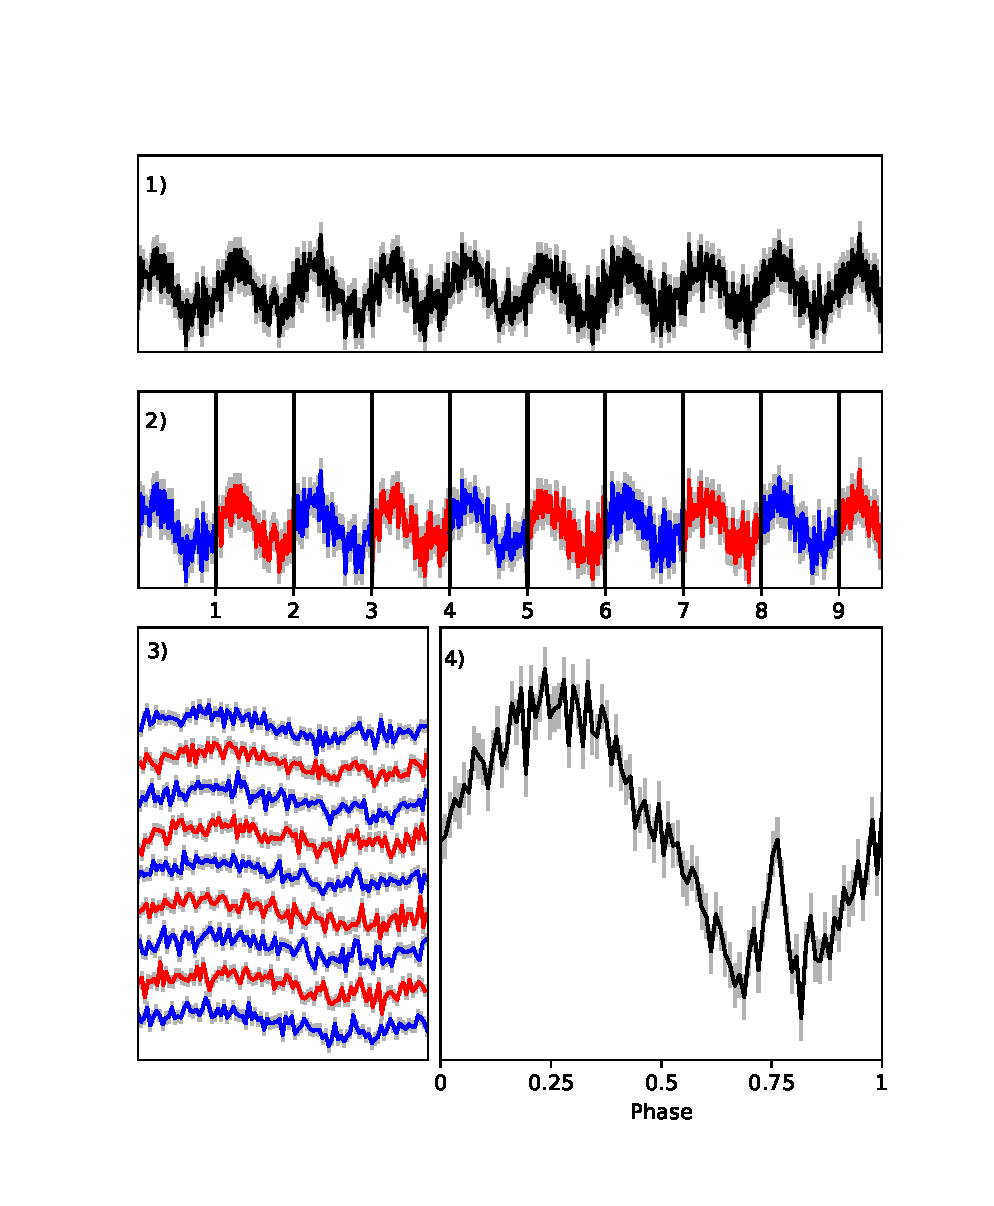
\includegraphics[width=\columnwidth, trim = 0mm 20mm 0mm 28mm]{images/folding.eps}
    \captionsetup{singlelinecheck=off}
    \caption[A cartoon illustrating the process of folding a periodic lightcurve with a known period.]{A cartoon illustrating the process of folding a periodic lightcurve with a known period.  \textbf{1:} a simulated lightcurve with errors.  \textbf{2:} Divide the lightcurve into sections by cutting it at every time coordinate $Np$, where $p$ is the known period and $N$ is any integer.  Each data point may now be given a phase coordinate $\phi$ in addition to its time coordinate $t$, where $\phi=(t/p)-N$ for $N$ such that $0\leq\phi<1$.  \textbf{3:} The lightcurve segments can be realigned in phase-space, such that points with the same value of $\phi$ sit at the same $x$-coordinate.  \textbf{4:} All points within given bins in $\phi$-space are averaged to create a lightcurve corresponding to the averaged oscillations of the original lightcurve.  The folding has revealed a peak at $\phi=0.75$ which was not apparent in the unfolded data.}
   \label{fig:Folding}
\end{figure}

\subsubsection{Flare-Finding Algorithm}
\label{sec:Flares}

\par To fold a quasi-periodic oscillation, such as the `heartbeat' flares seen in GRS 1915+105 and IGR J17091-3624, it is first important to find the $t$-values which characterise the beginning, end and peak of each flare.  To this end, I have created an algorithm to locate individual flares in a dataset containing non-periodic high-amplitude flares. The algorithm is performed as such (illustrated visually in Figure \ref{fig:BurstAlg}):

\begin{enumerate}
  \item Choose some threshold values $T_L$ and $T_H$.  Set the y-value of all datapoints with $y<T_L$ to zero.
  \item Retrieve the $t$-co-ordinate of the highest value remaining in the dataset.  Call this value $t_m$ and store it in a list.
  \item Set the value of point at $t_m$ to zero.
  \item Scan forwards from $t_m$.  If the selected point has a nonzero value, set it to zero and move to the next point.  If the selected point has a zero value, move to step 5.
  \item Scan backwards from $t_m$.  If the selected point has a nonzero value, set it to zero and move to the previous point.  If the selected point has a zero value, move to step 6.
  \item Retrieve the y-co-ordinate of the highest value remaining in the dataset.  Call this $y_m$.
  \item If $y_m>T_H$, repeat steps 2--7.  If $y_m<T_H$, proceed to step 8.
  \item Restore the original dataset.
  \item Retrieve the list of $t_m$ values found in step (ii).  Sort them in order of size.
  \item For each pair of adjacent $t_m$ values, find the $t$-coordinate of the datapoint between them with the lowest y-value.  Call these values $t_c$.
  \item This list of $t_c$ can now be used to demarcate the border between peaks.
\end{enumerate}

\begin{figure}
    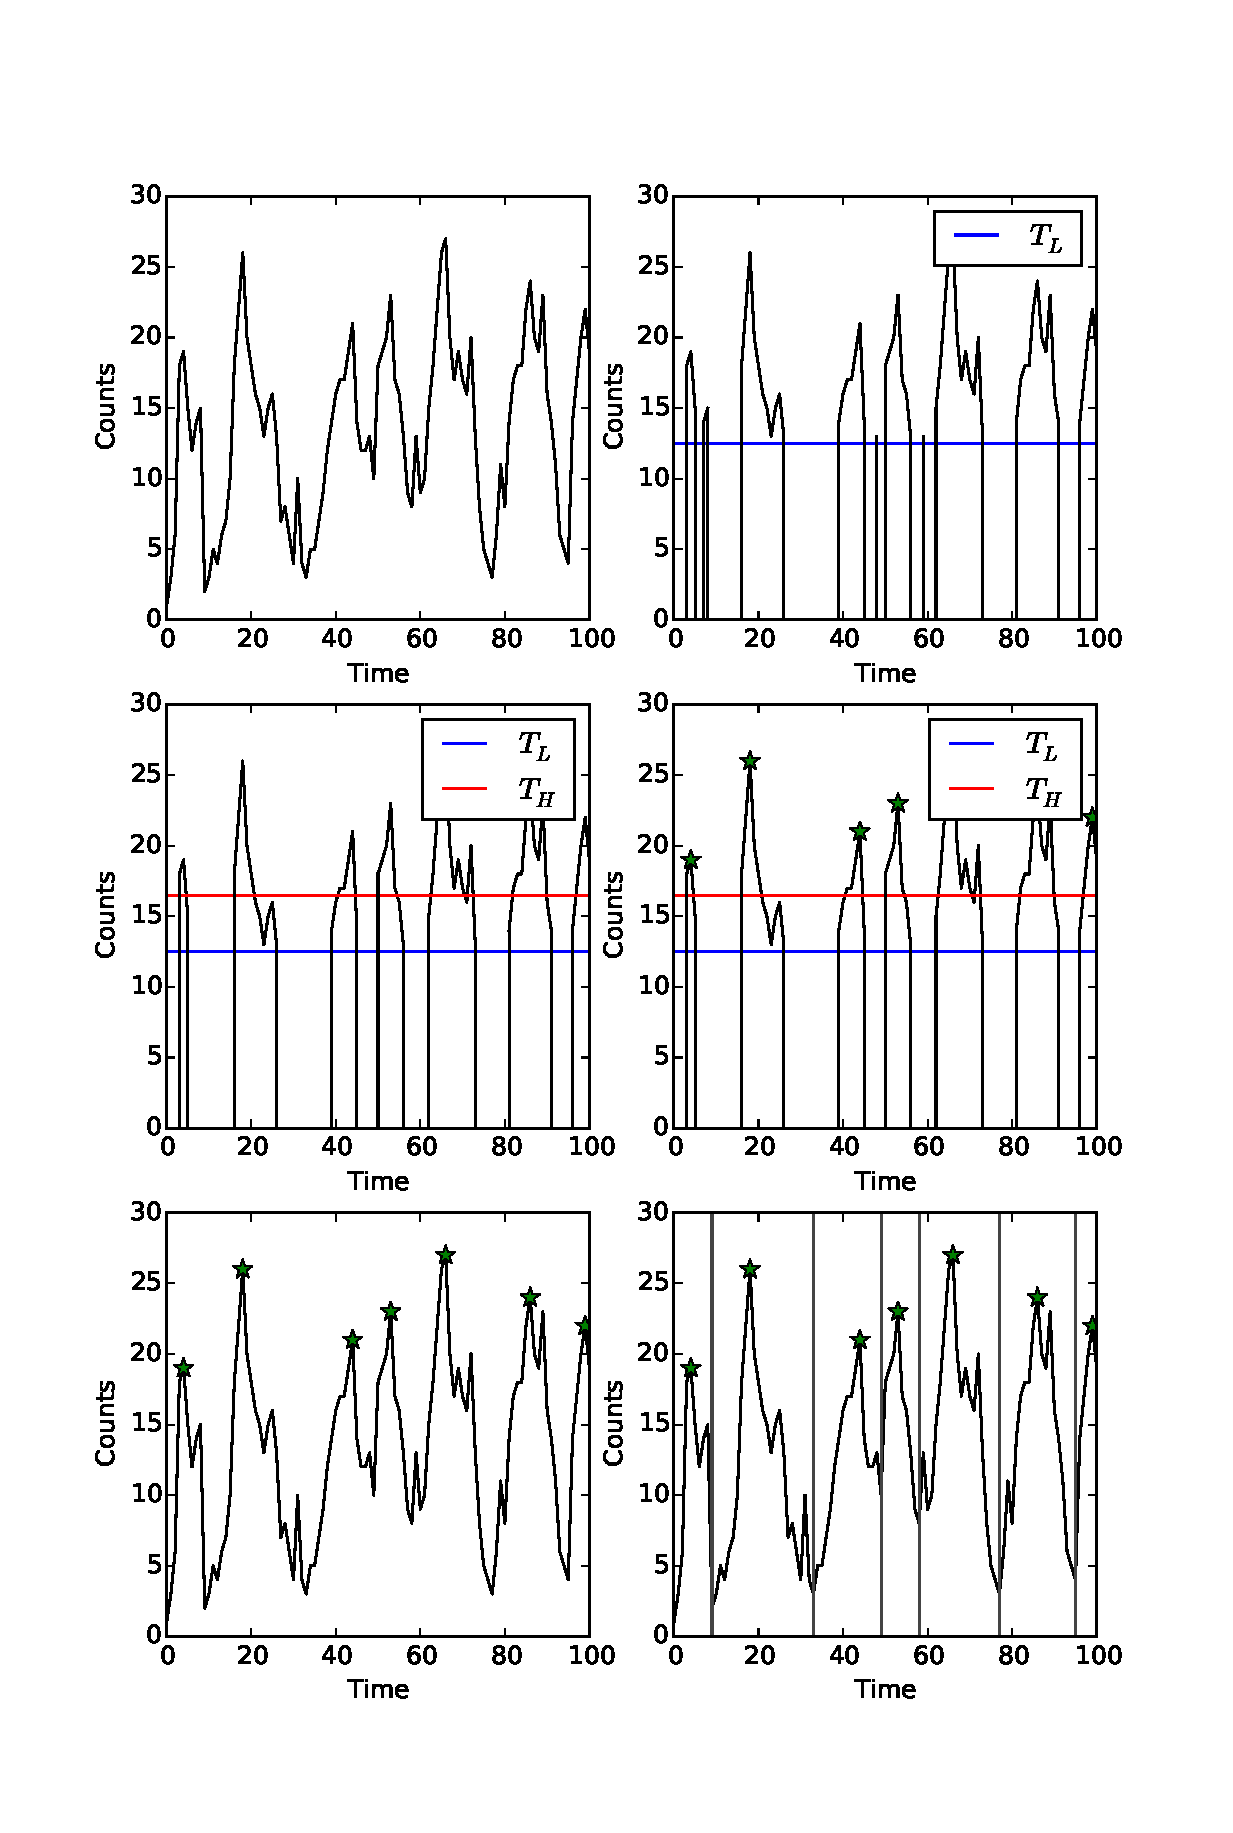
\includegraphics[width=\columnwidth, trim = 0mm 30mm 0mm 28mm]{images/steps.eps}
    \captionsetup{singlelinecheck=off}
    \caption[A cartoon illustrating the procedure of the algorithm described in Section \ref{sec:Flares}.]{From top-left: (i) An untouched data-set.  (ii) The dataset with all $y<T_L$ removed.  (iii) The dataset with all contiguous nonzero regions with $\max(y)<T_H$ removed.  (iv) The $t$-coordinates of peak $y$-values $t_m$.  (v) The restored dataset with the $t_m$ highlighted.  (vi) The boundaries between adjacent peaks.}
   \label{fig:BurstAlg}
\end{figure}

The values $T_L$ and $T_H$ can also be procedurally generated for a given piece of data:

\begin{enumerate}
  \item Select a small section of the dataset or a similar dataset (containing $\sim20$ peaks by eye) and note the time-coordinates $t_e$ of all peaks found by eye.
  \item Let $P_L$ and $P_H$ be two arbitrary values in the range $[0,100]$.
  \item Let $T_L$ ($T_H$) be the $P_L$th ($P_H$th) percentile of the y-values of the subsection of dataset.
  \item Run the flare-finding algorithm up to step 9.  Save the list of $t_m$.
  \item Split the dataset into bins on the x-axis such as the bin width $b\ll p$, where $p$ is the rough x-axis separation between peaks.
  \item For each bin, note if you found any value in $t_m$ falls in the bin and note if any value of $t_e$ falls in the bin.
  \item Using each bin as a trial, compute the Heidke Skill Score \citep{Heidke_SKSC} of the algorithm with the method of finding peaks by eye:
  \begin{equation}HSS = \frac{2(AD-BC)}{(A+B)(B+D)+(A+C)(C+D)}
  \label{eq:HSS}
  \end{equation}
  Where $A$ is the number of bins that contain both $t_e$ and $t_m$, $B$ ($C$) is the number of bins that contain only $t_m$ ($t_e$) and $D$ is the number of bins which contain neither \citep{Kok_YesNo}.
  \item Repeat steps (iii)--(vii) for all values of $P_H>P_L$ for $P_L$ and $P_H$ in $[1,100]$.  Use a sensible value for the resolution of $P_L$ and $P_H$.  Save the HSS for each pair of values
  \item Locate the maximum value of HSS, and note the $P_L$ and $P_H$ values used to generate it.  Use these values to generate final $T_L$ and $T_H$ values.
\end{enumerate}

I show an example of Heidke skill score grid for this algorithm, applied to a Class IV observation, in Figure \ref{fig:Heidke}.

\begin{figure}
    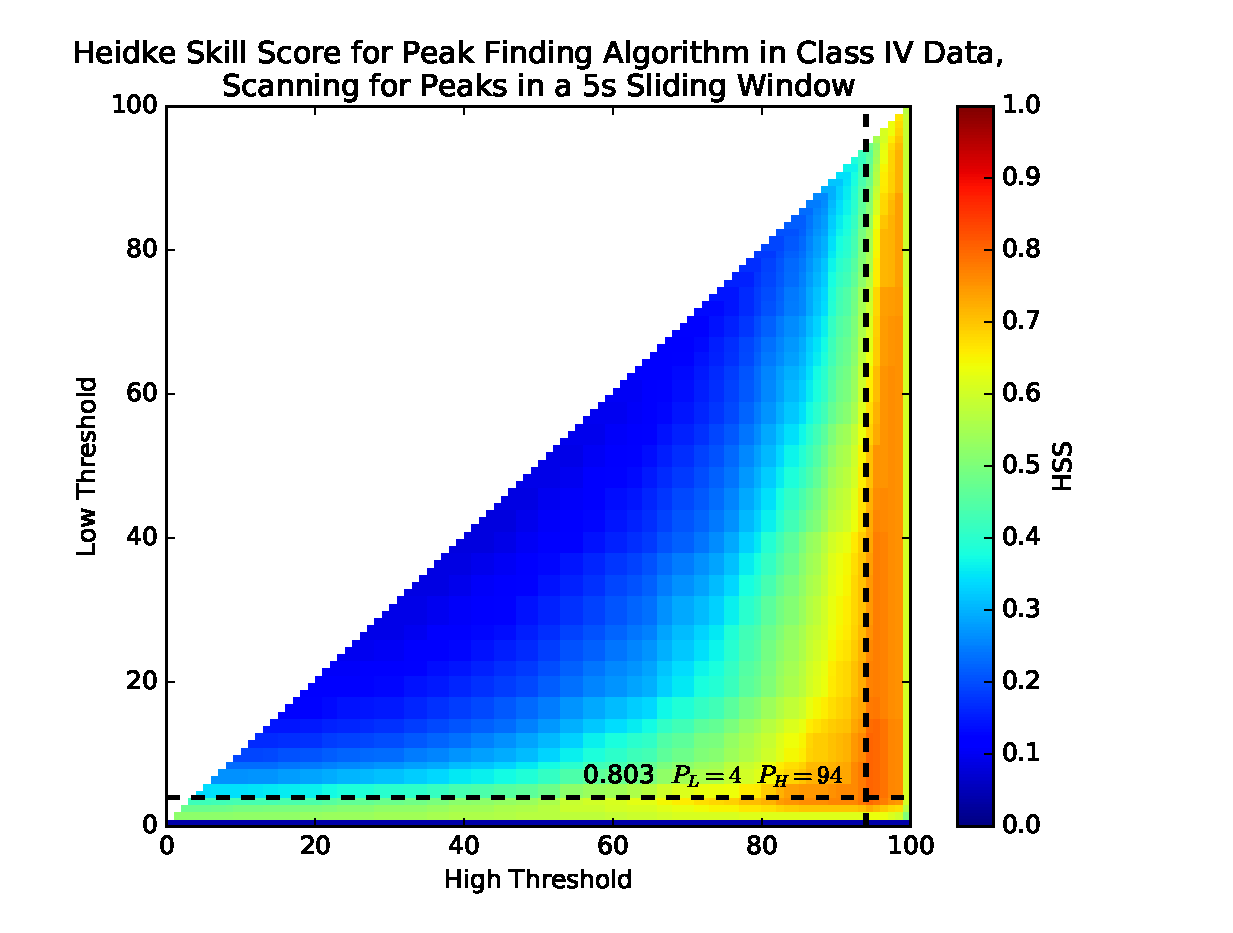
\includegraphics[width=\columnwidth, trim = 0mm 10mm 0mm 10mm]{images/HSS_J.eps}
    \captionsetup{singlelinecheck=off}
    \caption[The Heidke Skill score of a Class IV observation of IGR J17091-3624 for a selection of different values $P_L$ and $P_H$ (low and high threshold respectively).]{The Heidke Skill score of a Class IV observation of IGR J17091-3624 for a selection of different values $P_L$ and $P_H$ (low and high threshold respectively).}
   \label{fig:Heidke}
\end{figure}

\subsubsection{Variable Period Lightcurve Folding}

\par With the values $t_m$ and $t_c$ found using the algorithm described above, it is possible to recast Equation \ref{eq:simfold} to fold data over a high-amplitude but quasi-periodic oscillation.  I detail my method below:

\begin{enumerate}
  \item Take the ascending list of peak $t$-coordinates $t_m$.  Assign the first element a value $\Phi=0$.
  \item Assign each other point in $t_m$ an integer value $\Phi(t)$, such that the $\Phi$ value of the $i$th value of $t_m$ is defined as:
  \begin{equation}
  \Phi(t_m^{i})=\Phi(t_m^{i-1})+1, i\geq2
  \end{equation}
  \item If the troughs between bursts are well-defined, proceed to step 4.  Otherwise, skip to step 6.
  \item If the $t$-coordinate of the first datapoint in $t_c$ is less than the $t$-coordinate of the first datapoint in $t_m$, assign $\Phi(t_c^1)=-0.5$.  Otherwise, assign $\Phi(t_c^1)=-0.5$.
  \item Assign each other point in $t_m$ a value $\Phi(x)$, such that the $\Phi$ value of the $i$th value of $t_c$ is defined as:
  \begin{equation}
  \Phi(t_c^{i})=\Phi(t_c^{i-1})+1, i\geq2
  \end{equation}
  \item Create a general function defining $\Phi$ for all $t$ by fitting the $t$ and $\Phi$ values of $t_m$ (and $t_c$, if used) with a monotonically increasing univariate cubic spline\footnote{Computationaly realised as \texttt{PchipInterpolator} in the \texttt{scipy} package for Python \citep{NumPy}.} $S(t)$.
  \item Define the phase $\phi(t)$ of an arbitrary time $t$ as $\phi(t)=S(t)\mod1$.
\end{enumerate}

\par With a phase defined for all points in time, the data can be manipulated as if it had been folded in the usual way.  If the trough times in addition to the peak times are used to construct the spline, then the folded data are more accurate: however, by definition the rising part of each flare will occupy phases 0.5--1.0, while the falling part will occupy 0.0--0.5, so any assymetry in the rise and fall times of the average flare is lost.

\subsection{Timing Analysis}

\par Another way of looking at the variability of an astrophysical source is by looking in the frequency domain.  Well-established mathematical techniques, in particular Fourier spectroscopy, are able to deconvolve a time series into series of sine waves.  The amplitudes of these sine waves indicate how much variability in the system takes place at a given frequency.

\subsubsection{Fourier Spectroscopy}

\par Fourier Spectroscopy \citep{Fourier} is the most common way to perform frequency analysis on a time series.  The Fourier transform $\hat{f}(\nu)$ of a time series $f(t)$ is defined as:
\begin{equation}
\hat{f}(\nu)=\int_\infty^\infty f(t)e^{-2\pi it\nu} dt
\end{equation}
Where $\nu$ is the frequency to be probed and $i\equiv\sqrt{-1}$.  The magnitudes of the complex values $\hat{f}(\nu)$ describe the amplitude of the sine wave deconvolution at frequency $\nu$, while the arguments describe the relative phase of each of these sine waves.  As such, a plot of $|\hat{f}(\nu)|$ against $\nu$, known as a Fourier spectrum, highlights the frequencies at which the time series shows oscillations.  A strictly periodic oscillation shows up in a Fourier spectrum as a delta spike at a single frequency $\nu_p$; if the oscillation is not strictly sinusoidal, then there may also be spikes present at the harmonic frequencies $N\nu_p$ for any $N\in\mathbb{N}$.  A quasi-periodic oscillation shows up in a Fourier spectrum as a Lorentzian, defined by its amplitude and its quality factor $q$.  Quality factor is in turn defined as peak frequency divided by full-width half-maximum frequency width, and it represents approximately the number of oscillations over which the QPO remains coherent.
\par Fourier Spectroscopy was envisioned to analyse continuous, infinite data.  However, physical data differs from this ideal case in two important ways:
\begin{enumerate}
\item Physical data are discrete rather than continuous, consisting of samples taken at a finite rate $r$.
\item Physical data are finite rather than infinite, being taken in some window of length $w$.
\end{enumerate}
As such, as I show in Figure \ref{fig:convolve}, physical data consists of a time series convolved with both a windowing function and a sampling function.  Each of these convolutions adds spurious features to the power spectrum produced by the data.

\begin{figure}
    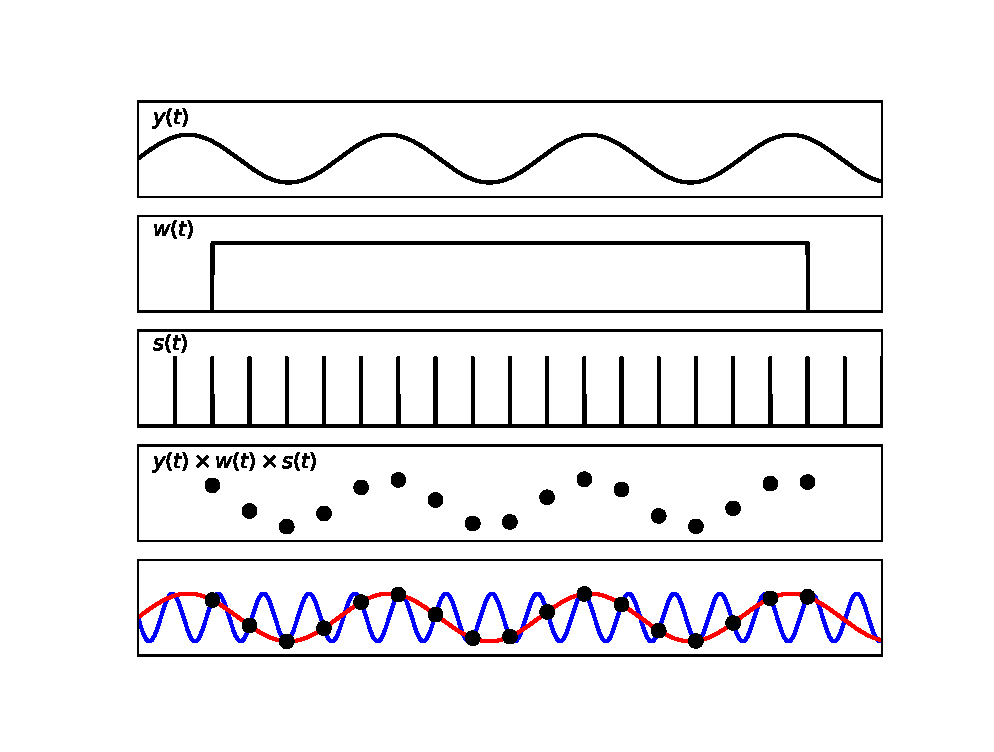
\includegraphics[width=\columnwidth, trim = 0mm 10mm 0mm 10mm]{images/convolve.eps}
    \captionsetup{singlelinecheck=off}
    \caption[A representation of how a continuous variable is convolved with a windowing function and a sampling function to yield physical data.]{A representation of how a continuous variable $y(t)$ is convolved with a windowing function $w(t)$ and a sampling function $s(t)$ to yield physical data.  The bottom panel shows how aliasing arises, showing that sine waves of two different frequencies can be fit to the data: one with a frequency $\nu$ equal to that in the original dataset, and one of frequency $\sigma-\nu$ where $\sigma$ is the sampling frequency.}
   \label{fig:convolve}
\end{figure}

\par The convolution with a sampling function adds so-called `aliased' peaks to the power spectrum of a given dataset.  For each peak in the power spectrum at frequency $\nu$, there will also be a peak present at a frequency of $\sigma-\nu$, where $\sigma$ is the sampling frequency.  This peak can be understood as the beat frequency between the oscillation in the data and the sampling frequency (see also the lower panel of Figure \ref{fig:convolve} for a visual explanation), and contains no additional information on the system.  To avoid these aliased peaks, values of $\hat{f}(\nu)$ outside of the range $0<\nu\leq\sigma/2$ are discarded.  The frequency $\sigma/2$, the maximum frequency at which one can extract useful information on a parameter sampled at constant frequency $\sigma$, is known as the Nyquist frequency.
\par The convolution with the windowing function causes peaks in the power spectrum to be broadened; an effect known as `spectral leakage'.  The form of this broadening depends on the windowing function which is being used.  Generally, physical data has been convolved with a so-called `boxcar' window; i.e., a function which takes a value of 1 during the period of measurement and 0 elsewhere.  A convolution with a boxcar window causes each peak in the power spectrum to be accompanied by a number of lower-amplitude sidelobes either side of it in frequency space; this serves to smear out a power spectrum and causes some information to be lost.  Other windows can be applied to data to attempt to lessen this effect; for example, convolving a dataset with a triangular or Gaussian windowinstead of a boxcar.  Many non-boxcar windows have been formulated to lessen the effect of spectral leakage, but it is impossible to remove the effect completely when working with a finite dataset.

\subsubsection{Fast Fourier Transform}

\par Taking the Fourier transform of a series is a computationally expensive procedure.  As such, it is common practice to instead use Fast Fourier Transform (FFT) algorithms; computationally fast algorithms which specialise in finding the Fourier transform of evenly-spaced series.
\par One such FFT algorithm is the Cooley-Tukey\footnote{Computationaly realised as \texttt{fft} in the \texttt{scipy.fftpack} package for Python \citep{NumPy}.} algorithm \citep{Cooley_FFT}.  The Cooley-Tukey algorithm speeds up the Fourier transform process by recursively dividing a datset in half to make many segments.  It uses the fact that the discrete Fourier transform of a single point is equal to itself, and then reconstructs the complete Fourier spectrum from these results. Unlike the basic Fourier transform, the Cooley-Tukey algorithm is only able to transform series which are evenly spaced in time and consisting of $2^N$ datapoints, for $N\in\mathbb{N}$.
\par The error on a Fast Fourier Transform of an arbitrary dataset is 100\%.  There are two ways to reduce this error to a level at which the data can be meaningfully analysed:
\begin{enumerate}
\item The original time series can be split into a number of equal-length windows.  The Fast Fourier-Transforms of these windows can be calculated independently of each other, and then averaged to create the mean FFT of the dataset.
\item The resultant power spectrum can be rebinned in frequency space.
\end{enumerate}
\par Propagating errors in the usual way, this results in a final error on Fourier power $\delta\hat{f}(\nu)$ of:
\begin{equation}
\delta\hat{f}(\nu)=\frac{\hat{f}(\nu)}{\sqrt{MW}}
\end{equation}
Where $W$ is the number of windows the original dataset was divided into, and $M$ is the number of frequency bins which were averaged to obtain the Fourier power at frequency $\nu$.  Increasing $W$ increases the minimum frequency at which the Fourier power of the dataset can be probed, while increasing $M$ removes information on the fine structure of the power spectrum.

\subsubsection{Normalising the Fourier Transform}

\par To understand the significance of features in a power spectrum, it is important to normalise the results in a standard and well-understood way.  One such method of normalisation is the `Leahy' normalisation \citep{Leahy_Norm}, defined as:
\begin{equation}
L(\nu)=\frac{2\times|\hat{f}(\nu)|^2}{n_{p}}
\end{equation}
Where $n_p$ is the total number of photon counts in the original dataset.  This normalisation has the property that pure Poisson noise has a Leahy-normalised power of 2\footnote{In practise, due to instrumental dead-time effects meaning photon arrivals are not strictly independent, Poisson noise in astrophysical data tends to yield a Leahy-normalised power of slightly less than 2}.
\par I use one additional power spectrum normalisation in the work presented in this thesis: the RMS normalisation.  This is defined as:
\begin{equation}
R(\nu)=\frac{(L(\nu)-2)r_s}{(r_s-r_b)^2}=\frac{2\left(|\hat{f}(\nu)|^2-Tr_s\right)}{T(r_s-r_b)^2}
\end{equation}
\par Where $T$ is the total time duration of all data used to produce the power spectrum, $r_s$ is the mean source count rate and $r_b$ is the mean background rate.  In this normalisation, Poisson noise corresponds to a power of zero.  Additionally, the power spectrum has the property that the integral of $R(\nu)$ between two frequencies is equal to the root-mean squared amplitude of the variability of the original time series in that frequency band.

\subsubsection{Lomb-Scargle Periodograms}

\par Fast Fourier transforms are unable to process unevenly spaced time series.  Additionally, while mathematical Fourier transforms can in general process unevenly spaced datasets, the effects of aliasing become increasingly complex and difficult to disentangle from real signal.  In these cases, a method known as the Lomb-Scargle periodogram, based on proposals by \citet{Lomb_LombScargle} and \citet{Scargle_LombScargle}, can be used.
\par The Lomb-Scargle periodogram can be thought of as the result of fitting sinusoids of frequency $\nu$ to a time series, and constructing a spectrum using the $\chi^2$ value of the fit of the sinusoid at each $\nu$.  Unlike a Fourier spectrum of unevenly spaced data, the Lomb-Scargle periodogram of unevenly spaced data is statistically well-behaved as long as the white-noise component of the dataset is uncorrelated.
\par Unfortunately, due to dead-time effects present in all X-ray telescopes, white noise in real datasets is not uncorrelated and so the statistical properties of the Lomb-Scargle spectrogram are generally not well-defined.  In this case, bootstrapping techniques can be used to estimate the significances of features in the power spectrum.

\subsection{Energy Spectral Analysis}

\par Energy spectral analysis is perhaps the most powerful tool available to understand the physical processes at work in astrophysical systems.  The distribution of arriving photons as a function of energy can be fit to physical models which, assuming a given system geometry, can provide estimates of various system parameters.
\par The disadvantage of spectral fitting is the aforementioned assumptions that one has to make.  A number of well-studied spectral models of LMXBs exist, which are able to return estimates for values such as inner disk radius, black hole mass and spin when fit to data.  However, the values that different models return often contradict each other, and thus the values that a study infers for these parameters depends heavily on the system physics and geometry that the modeller assumes.

\subsubsection{Hardness-Intensity Diagrams}

\label{sec:hids}

\par A model-independent way to study the spectral properties of a source is by using `hardness'.  To obtain the hardness of a source, first define two non-overlapping energy bands $A$ and $B$ with $B>A$.  The hardness is then defined as $H(t)=r_B(t)/r_A(t)$, where $r_x(t)$ is the photon arrival rate in some band $x$.  The hardness gives basic information on the shape of the energy spectrum without assuming a physical model.
\par Hardness is often paired with intensity (i.e. $r_A(t)+r_B(t)$) to create `hardness-intensity diagrams' (HIDs) to explore how the source spectrally varies over time.  To explain what the shape of an HID diagram can tell us about the spectral evolution of a source, consider the following examples of HIDs for a black body spectrum with temperature $T(t)$ and normalisation $n(T)$:
\begin{enumerate}
\item $T(t)=1, n(t)=\sin(t)$: in this example, the brightness of the source changes over time but the shape of its spectrum does not change.  As such the hardness is a constant, and the system traces a vertical line in hardness-intensity space (Figure \ref{fig:HIDexp}, Panel 1).
\begin{figure}
    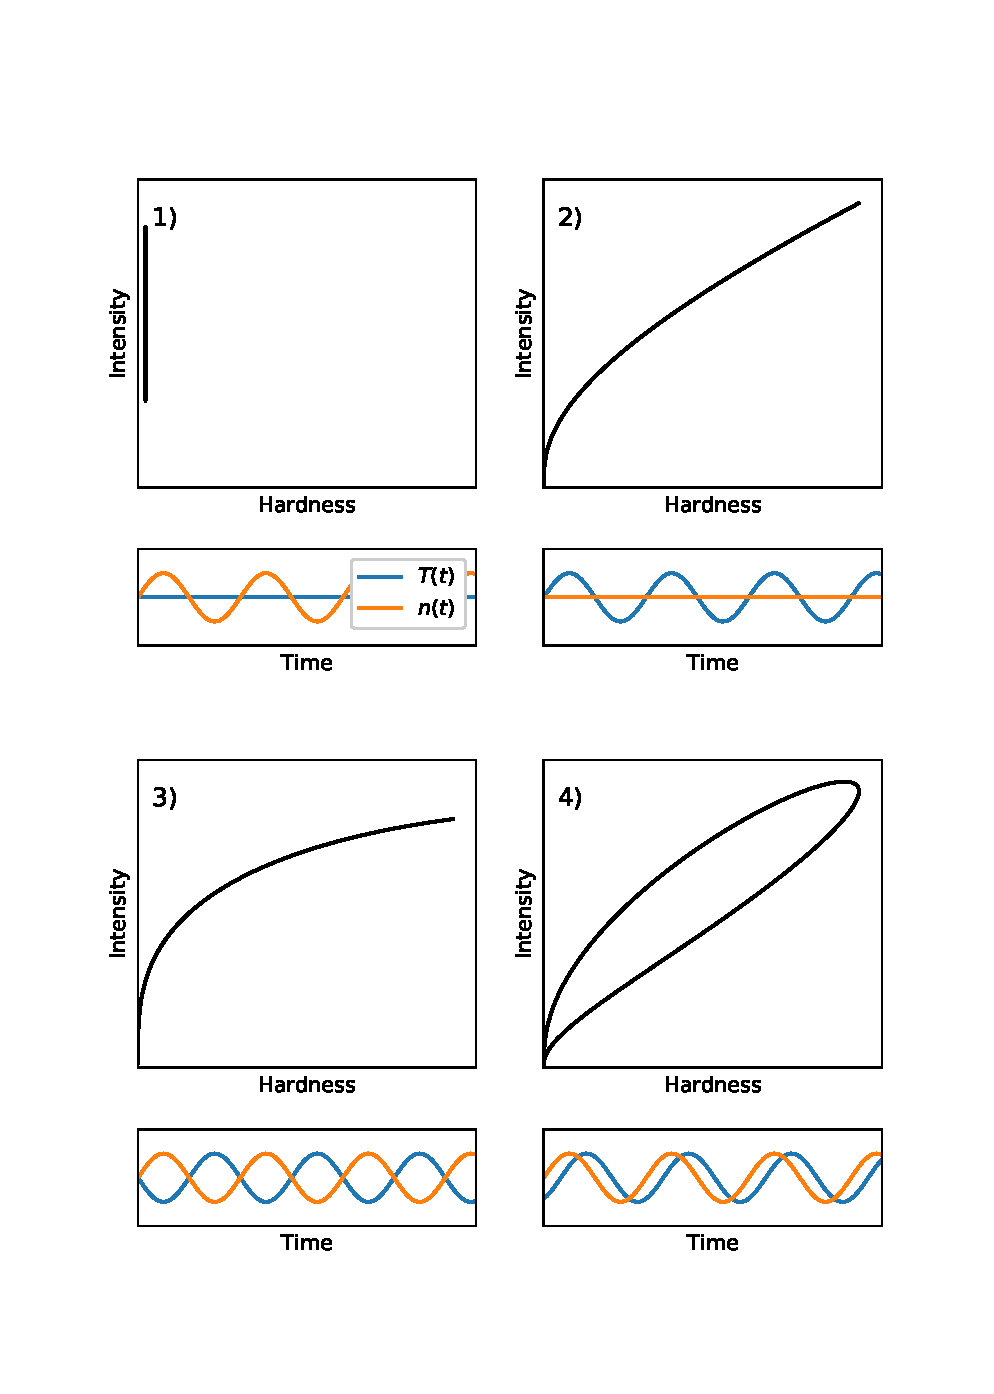
\includegraphics[width=\columnwidth, trim = 0mm 25mm 0mm 25mm]{images/hidexp.eps}
    \captionsetup{singlelinecheck=off}
    \caption[Hardness-Intensity diagrams of black bodies with temperatures and normalisations described by various functional forms.]{Hardness-Intensity diagrams of black bodies with temperatures and normalisations described by various functional forms $T(t)$ and $n(t)$.  The plots show how HIDs differ between sources with \textbf{1)} changing brightness but no spectral change, \textbf{2)} changing temperature, \textbf{3)} changing temperature and normalisation in antiphase, and \textbf{4)} changing temperature and normalisation out of phase.}
   \label{fig:HIDexp}
\end{figure}
\item $T(t)=\sin(t), n(t)=1$: in this example, the spectrum of the source changes over time, resulting in a curved track in hardness-intensity space (Figure \ref{fig:HIDexp}, Panel 2).
\item $T(t)=\sin(t), n(t)=\sin(t-\pi)$: if two or more spectral parameters are varying at once, the track can become move complex.  If these parameters are varying in phase or antiphase, a single track is traced (Figure \ref{fig:HIDexp}, Panel 3).
\item $T(t)=\sin(t), n(t)=\sin\left(t+\frac{\pi}{3}\right)$: when parameters are varying out of phase with each other, the track of the object in a HID can take the form of a closed loop (Figure \ref{fig:HIDexp}, Panel 4).
\end{enumerate}
Case 4 is interesting, as it indicates the presence of a time lag between two or more physical components of the system.  The direction in which the loop is executed over time can be used to infer the sign of this lag.  This in turn can give constraints on the causal links between components of a system, in turn giving constraints on physical models proposed to describe them.

\subsubsection{Phase-Resolved Spectroscopy}

\label{sec:phasresspec}

\par Like lightcurves, HIDs and time-resolved spectra can be difficult to analyse when constructed from data with poor statistics.  If the source is variable in a periodic or quasi-periodic way, a modified version of the folding algorithms detailed in Section \label{sec:LCMorph} can be used to analyse the spectral evolution of an average cycle:
\begin{itemize}
\item Obtain the function $\phi(t)$ to describe how phase varies as a function of time.
\item Split the interval $[0,1)$ into a number of sub-intervals $i$.
\item For each sub-interval $i$, compile a list of good time indices (GTIs) denoting periods of time during which $\phi(t)\in i$.
\item For each list of GTIs, filter the original dataset such that it only contains photons which arrived during one of the intervals.
\item From each new filtered dataset, a spectrum or hardness ratio can be calculated.  This can be compared with the spectra or hardness ratios taken from the other filtered datasets to analyse how the spectrum of the source varies as a function of phase.
\end{itemize}



